%%%%%%%%%%%%%%%%%%%%%%%%%%%%%%%%%%%%%%%%%%%%%%%%%%%%%%%%%%%%%%%%%%%%%%%%%%%
%
% Plantilla para un artículo en LaTeX en español.
%
%%%%%%%%%%%%%%%%%%%%%%%%%%%%%%%%%%%%%%%%%%%%%%%%%%%%%%%%%%%%%%%%%%%%%%%%%%%



%--------------------------------------------------------------------------
\title{Plantilla para un artículo \LaTeX}
\author{El autor va aquí\\
  \small Dept. Plantillas y Editores\\
  \small E12345\\
  \small España
}

\begin{document}
\maketitle

\abstract{En los últimos años, las organizaciones han recurrido cada vez más a soluciones de software avanzadas para administrar las cargas de trabajo, mantener la rentabilidad y asegurar la competitividad dentro de sus respectivas industrias. Si bien hay varias opciones disponibles, las herramientas de inteligencia de negocios (BI) y las herramientas de análisis de negocios (BA) son posiblemente las soluciones de administración de datos más implementadas. Los analistas de negocios y los compradores de software a menudo preguntan cuáles son las diferencias clave entre la inteligencia de negocios y los análisis de negocios.}
\\
\abstract{In recent years, organizations have increasingly turned to advanced software solutions to manage workloads, maintain profitability and ensure competitiveness within their respective industries. While there are several options available, business intelligence tools (BI) and business analytics tools (BA) are arguably the most widely implemented data management solutions. Business analysts and software buyers alike often ask what are the key differences between business intelligence vs business analytics.}

\section{Introduccion}

Las soluciones de inteligencia empresarial se encuentran entre las herramientas de administración de datos más valiosas disponibles. Las soluciones de BI recopilan y analizan datos actuales y procesables con el fin de proporcionar información para mejorar las operaciones comerciales. ¿Está buscando formas de entender mejor sus operaciones comerciales? ¿Qué hay de descubrir puntos de dolor en sus flujos de trabajo? ¿Qué hay de analizar grandes conjuntos de datos para obtener información valiosa? Necesita una solución de inteligencia de negocios.
\begin{center}
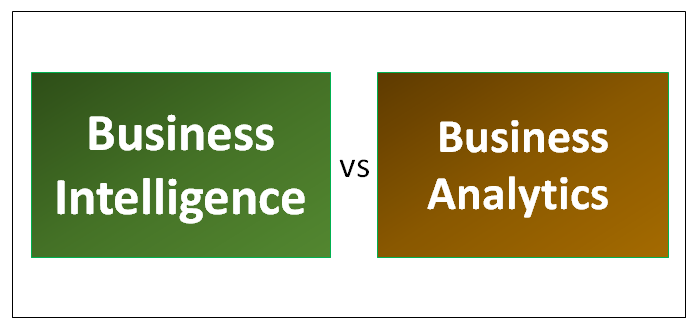
\includegraphics[width=10cm]{./Imagenes/bivsba}
\end{center}
El software de análisis de negocios es un niño o padre (dependiendo de a quién le pregunte) de la categoría de inteligencia empresarial. Al igual que BI, se utiliza principalmente para analizar datos históricos, pero con la intención de predecir las tendencias de negocios. Por lo general, también tiene un ojo hacia la mejora y la preparación para el cambio. 

\section{Marco teorico}
\title{BUSINESS INTELLIGENCE}\\\\
La Inteligencia de Negocios BI (Business Intelligence) es una herramienta bajo la cual diferentes tipos de organizaciones, pueden soportar la toma de decisiones basadas en información precisa y oportuna; garantizando la generación del conocimiento necesario que permita escoger la alternativa que sea más conveniente para el éxito de la empresa.\\\\
\begin{figure}[htb]
\begin{center}
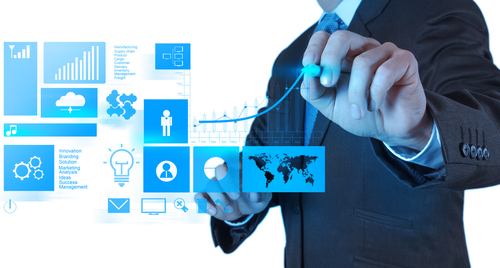
\includegraphics[width=10cm]{./Imagenes/inegocios}
\end{center}
\end{figure}
Desde un punto de vista más pragmático, y asociándolo directamente con las tecnologías de la información, podemos definir Business Intelligence como el conjunto de metodologías, aplicaciones y tecnologías que permiten reunir, depurar y transformar datos de los sistemas transaccionales e información desestructurada (interna y externa a la compañía) en información estructurada, para su explotación directa (reporting, análisis OLTP / OLAP, alertas...) o para su análisis y conversión en conocimiento, dando así soporte a la toma de decisiones sobre el negocio.\\\\
Los principales productos de Business Intelligence que existen hoy en día son:

*  Cuadros de Mando Integrales (CMI)

*  Sistemas de Soporte a la Decisión (DSS)

*  Sistemas de Información Ejecutiva (EIS)
\\\\
\title{BUSINESS ANALYTICS}\\\\
El análisis de negocio(Business Analytics, BA) es el conjunto de métodos y técnicas utilizadas para trabajar como enlace entre los stackeholders, con el fin de comprender la estructura, políticas y operaciones de una organización y recomendar soluciones que permitan a la organización alcanzar sus objetivos (IIBA: International Institute of Business Analysis).\\\\
El análisis de negocios implica la comprensión de cómo funcionan las organizaciones para llevar a cabo sus propósitos, y la definición de las capacidades que una organización requiere para proporcionar productos y servicios a los grupos de interés externos. Incluye la definición de los objetivos de la organización, cómo esos objetivos se conectan a objetivos específicos, que determinan las líneas de acción que una organización tiene que realizar para alcanzar esas metas y objetivos, y definir cómo las distintas unidades de organización y las partes interesadas dentro y fuera de esa organización interactúa.

\begin{figure}[htb]
\begin{center}
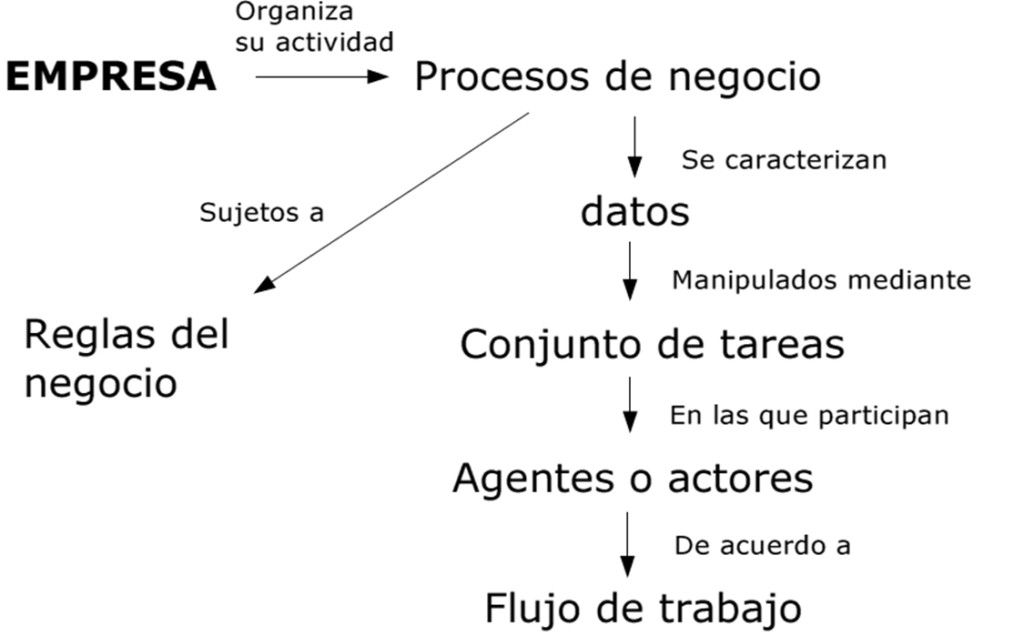
\includegraphics[width=10cm]{./Imagenes/anegocios}
\end{center}
\end{figure}

\section{Aplicacion}

Aquí va el texto.
\begin{equation}\label{eq:area}
  S = \pi r^2
\end{equation}
Uno puede referirse a ecuaciones así: ver ecuación (\ref{eq:area}).
También se pueden mencionar secciones de la misma forma: ver sección
\ref{sec:nada}. O citar algo de la bibliografía: \cite{Cd94}.



\subsection{Aplicaciones de BuBusiness Intelligence } \label{sec:nada}


Las herramientas de inteligencia de negocio son aplicaciones digitales diseñadas para colaborar con el Business Intelligence durante el análisis y la presentación de datos.\\
La Inteligencia de Negocios o Business Intelligence (BI) permite a las compañías contar con la información adecuada para una mejor toma de decisiones.  Las compañías que implementan el BI logran sacar mayor provecho de las situaciones de crisis gracias a la posibilidad de contar con un análisis de mercado más acertado debido a que los datos pesados son transformados en importantes estrategias corporativas.
Actualmente, las herramientas de BI disponibles en el mercado son incontables, pero estas 20 no pueden pasar desapercibidas:

\subsubsection{Microsoft Dynamics NAV: }\label{sec:nada2} 
Especial para pequeñas y medianas empresas que buscan mejorar su competitividad.
	\begin{center}
	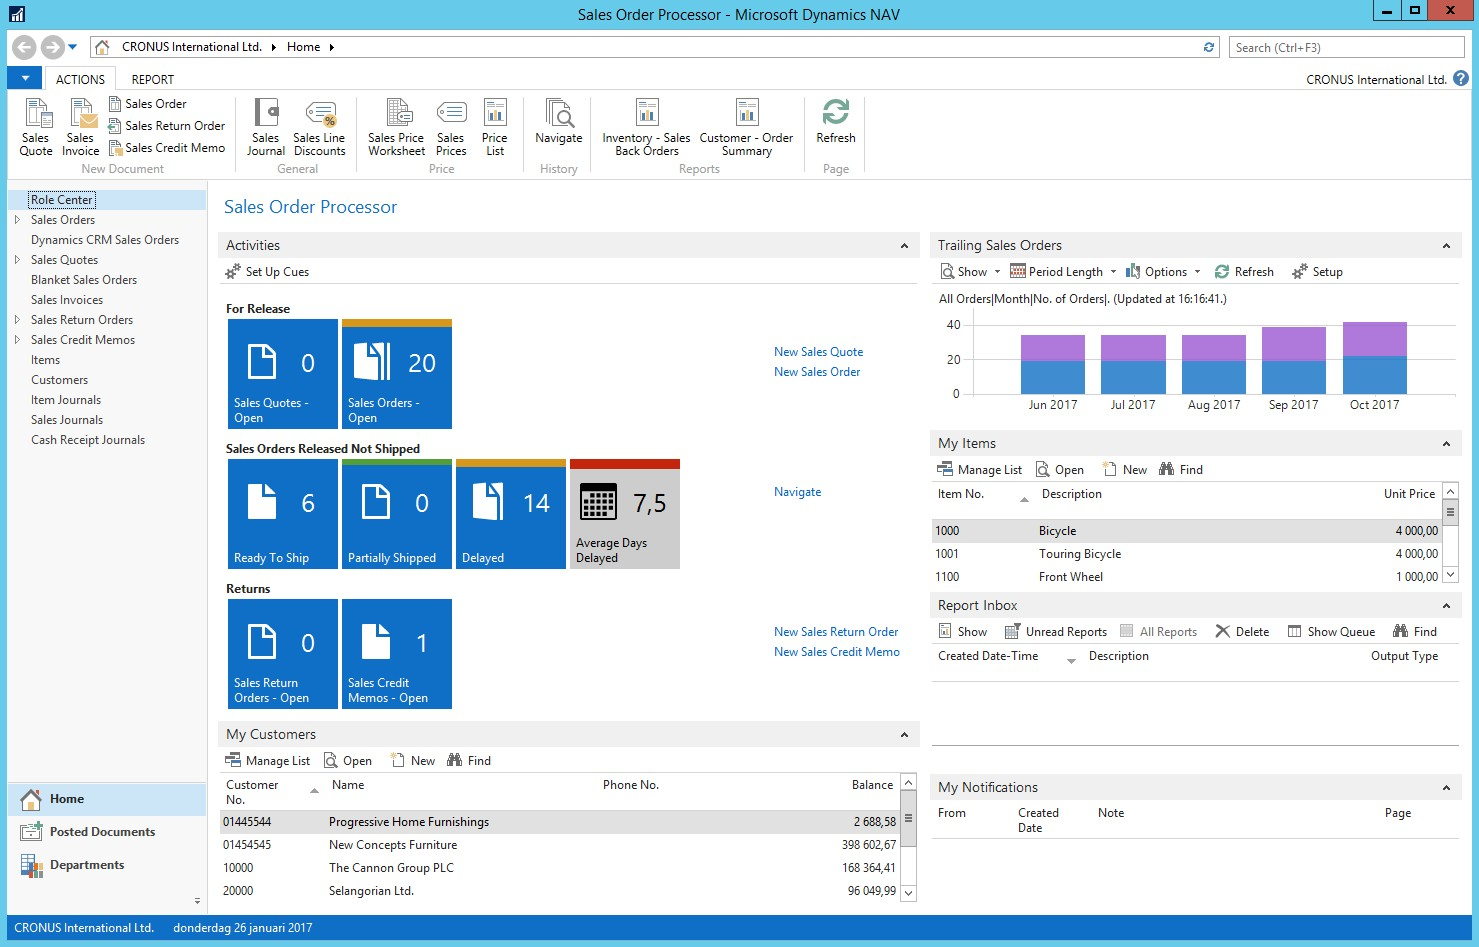
\includegraphics[width=15cm]{./Imagenes/BIimagen1}
	\end{center}

\subsubsection{Microsoft Dynamics CRM: }\label{sec:nada2}  
Efectiva para la administración de clientes.
	\begin{center}
	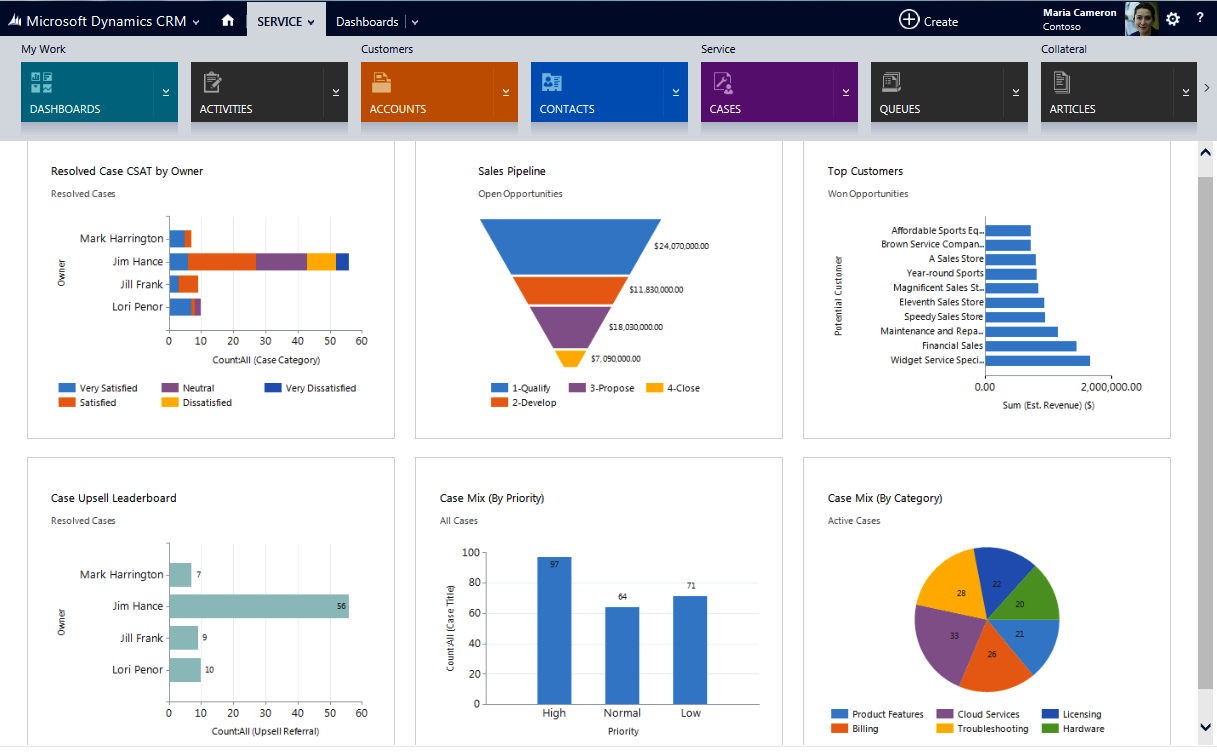
\includegraphics[width=15cm]{./Imagenes/BIimagen2}
	\end{center}
	
\subsubsection{Oracle Business Intelligence: }\label{sec:nada2} 
Una de las más completas en el mercado ya que cuenta con paneles interactivos, análisis predictivos en tiempo real, entre otros.
	\begin{center}
	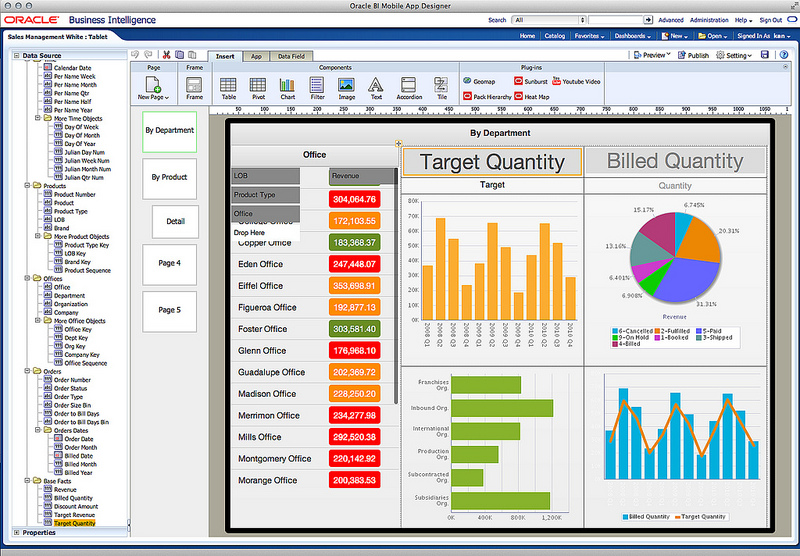
\includegraphics[width=15cm]{./Imagenes/BIimagen3}
	\end{center}
	
\subsubsection{Ultimus: }\label{sec:nada2}  
Un entorno integrado que permite compartir información entre aplicaciones.
	\begin{center}
	
\includegraphics[width=15cm]{./Imagenes/BIimagen4}
	\end{center}
	
\subsubsection{Office SharePoint Server: }\label{sec:nada2}  
Facilita el acceso a la información en cualquier momento y lugar.
	\begin{center}
	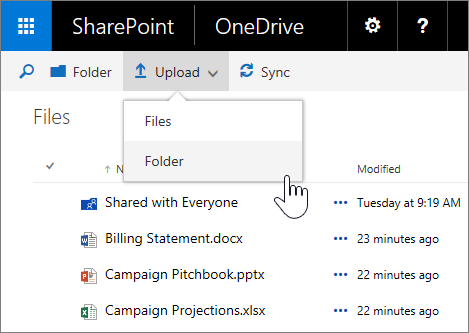
\includegraphics[width=15cm]{./Imagenes/BIimagen5}
	\end{center}
	
\subsubsection{QlikView: }\label{sec:nada2}  
Mantiene las bases de datos al alcance de una manera sin precedentes.
	\begin{center}
	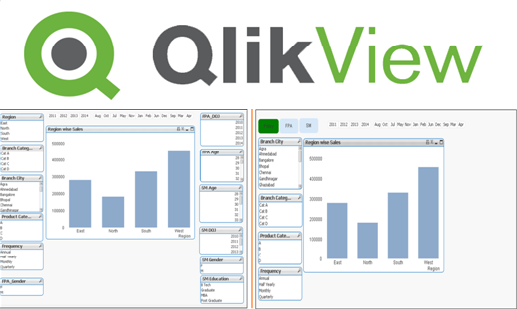
\includegraphics[width=15cm]{./Imagenes/BIimagen6}
	\end{center}
	
\subsubsection{Microsoft Performance Point Server: }\label{sec:nada2}  
Permite supervisar, alinear y hacer un plan de negocio.
	\begin{center}
	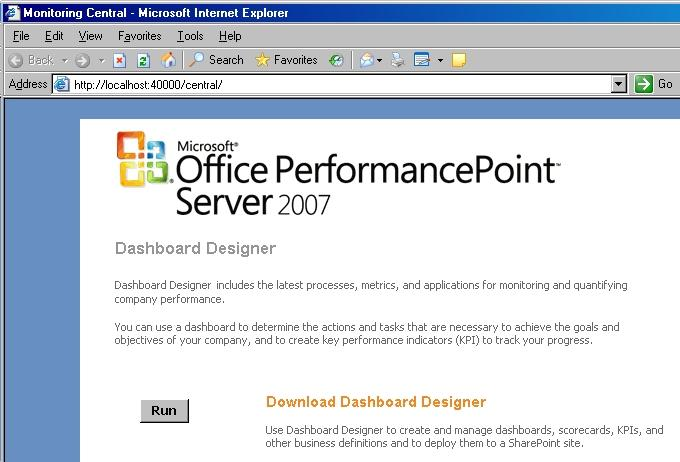
\includegraphics[width=15cm]{./Imagenes/BIimagen7}
	\end{center}
	
\subsubsection{Microsoft SQL Server: }\label{sec:nada2}  
Adecuada para realizar un análisis panorámico de la empresa y tomar las mejores decisiones.
	\begin{center}
	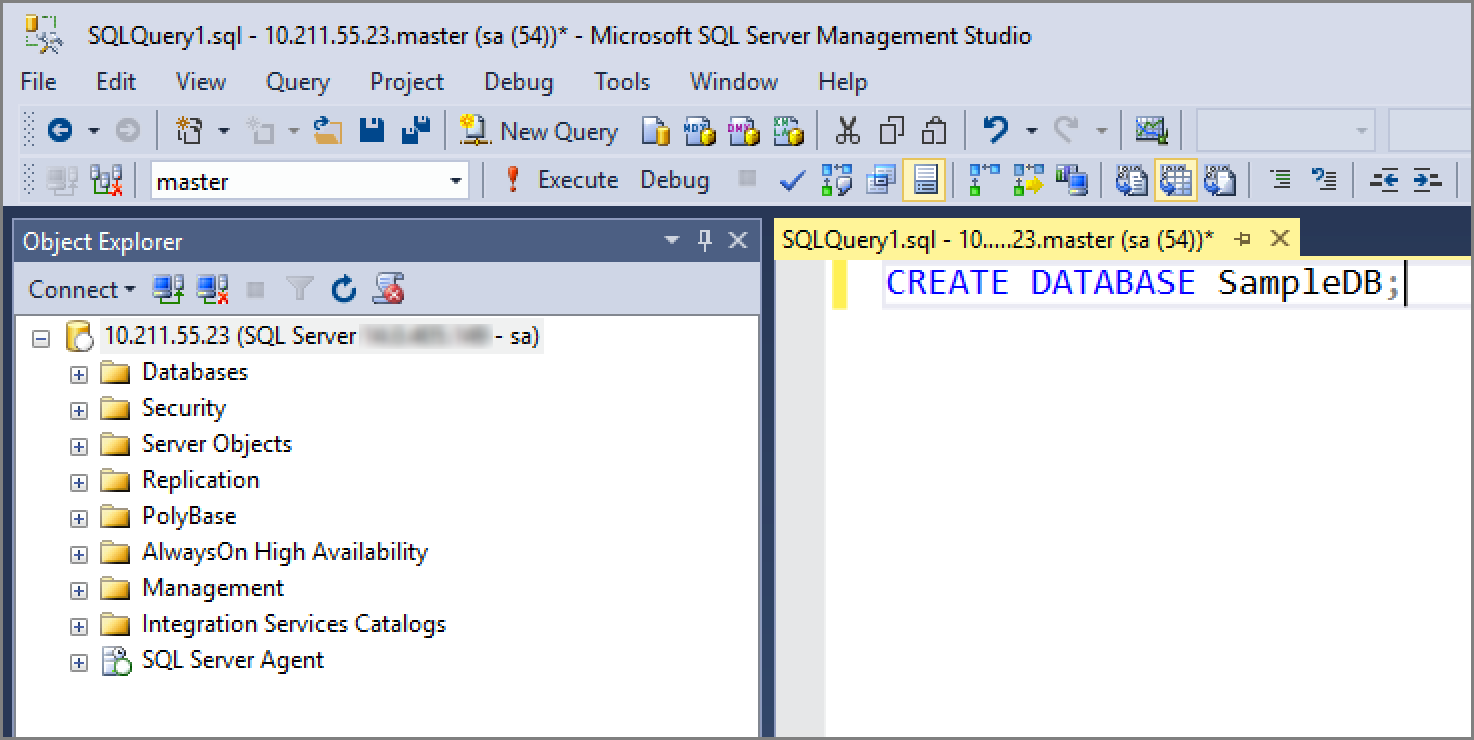
\includegraphics[width=15cm]{./Imagenes/BIimagen8}
	\end{center}
	
\subsubsection{JetReports: }\label{sec:nada2}  
Especial para crear informes ERP.
	\begin{center}
	
\includegraphics[width=15cm]{./Imagenes/BIimagen9}
	\end{center}
	
\subsubsection{Eclipse BIRT Project: }\label{sec:nada2}  
Genera informes para aplicaciones web de código abierto.
	\begin{center}
	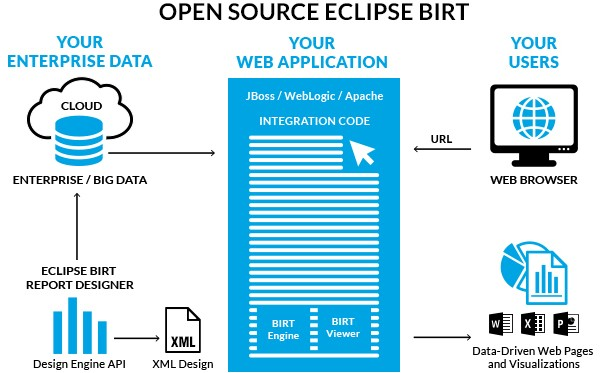
\includegraphics[width=15cm]{./Imagenes/BIimagen10}
	\end{center}
	
\subsubsection{JasperReports: }\label{sec:nada2}  
Permite crear informes de rápida impresión.
	\begin{center}
	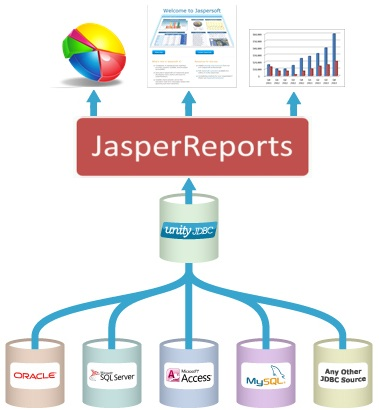
\includegraphics[width=15cm]{./Imagenes/BIimagen11}
	\end{center}
	
\subsubsection{LogiReport: }\label{sec:nada2}  
Aplicación gratuita basada en web de LogiXML
	\begin{center}
	
\includegraphics[width=15cm]{./Imagenes/BIimagen12}
	\end{center}
	
\subsubsection{OpenI: }\label{sec:nada2} 
Aplicación web orientada al reporting OLAP.
	\begin{center}
	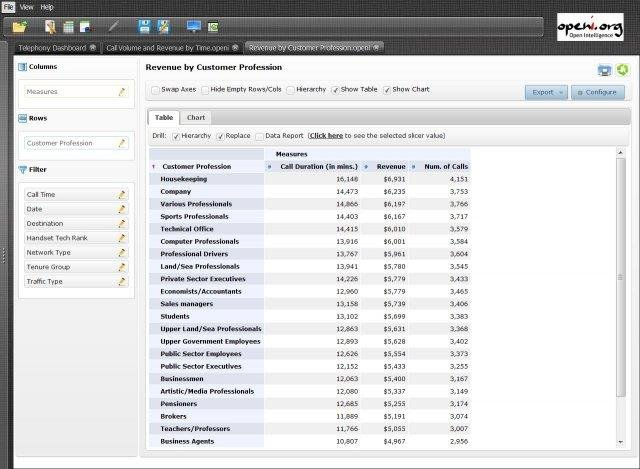
\includegraphics[width=15cm]{./Imagenes/BIimagen13}
	\end{center}
	
\subsubsection{SPSS: }\label{sec:nada2}  
Programa estadístico especialmente empleado en ciencias sociales e investigaciones de mercado.
	\begin{center}
	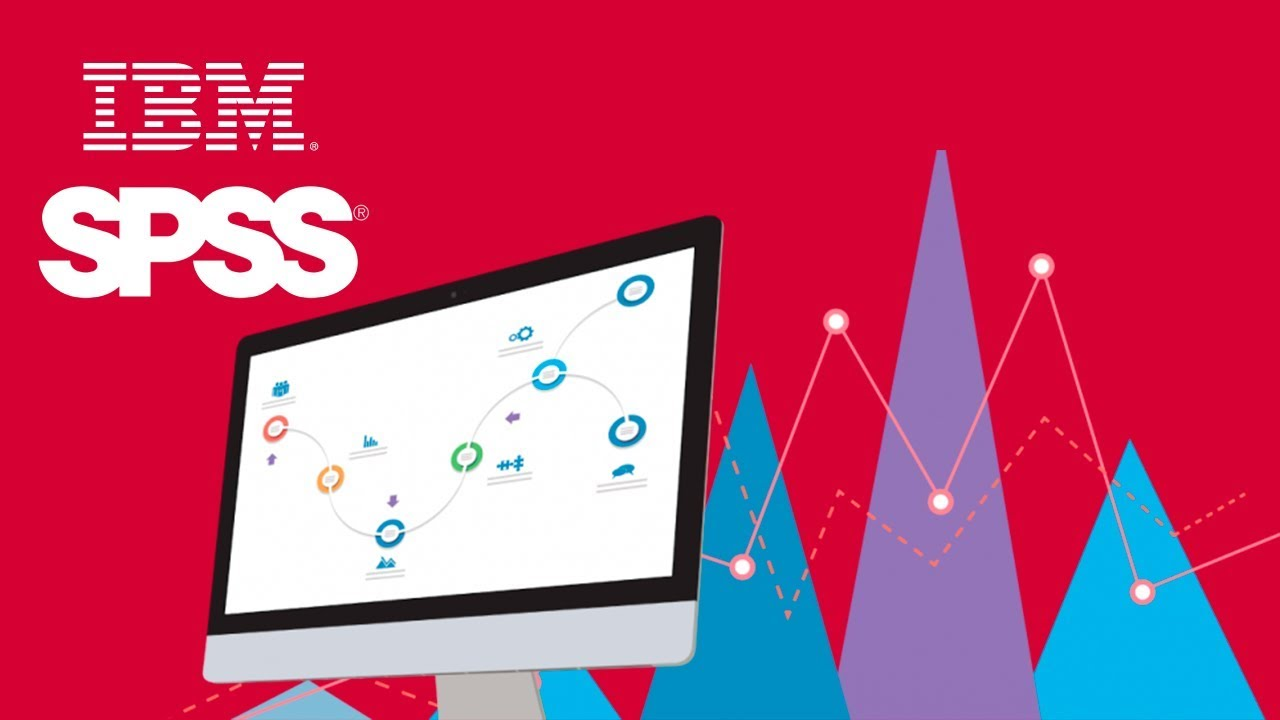
\includegraphics[width=15cm]{./Imagenes/BIimagen14}
	\end{center}
	
\subsubsection{Pentaho: }\label{sec:nada2}  
Incluye herramientas para generar informes, minería de datos, ETL, entre otros.
	\begin{center}
	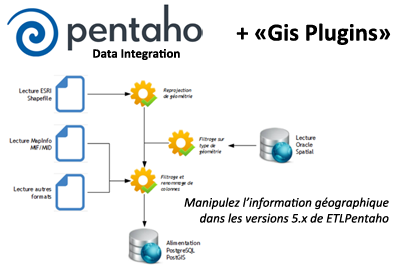
\includegraphics[width=15cm]{./Imagenes/BIimagen15}
	\end{center}
	
\subsubsection{RapidMiner: }\label{sec:nada2}  
Permite analizar datos a través de un entorno gráfico.
	\begin{center}
	
\includegraphics[width=15cm]{./Imagenes/BIimagen16}
	\end{center}
	
\subsubsection{Crystal Reports: }\label{sec:nada2}  
Genera informes desde bases de datos múltiples.
	\begin{center}
	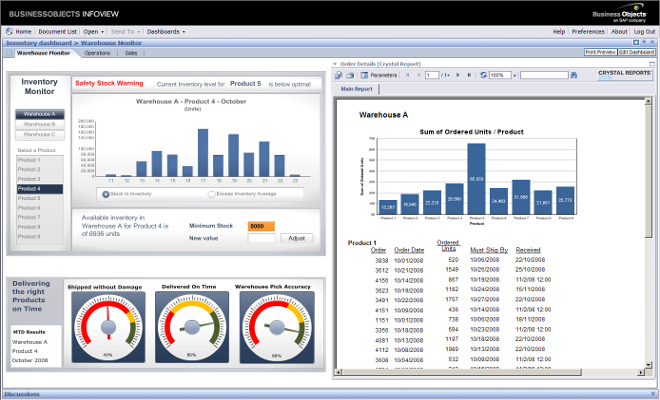
\includegraphics[width=15cm]{./Imagenes/BIimagen17}
	\end{center}
	
\subsubsection{ApeSoft: }\label{sec:nada2}  
Ofrece una interface sencilla similar a Microsoft Excel.
	\begin{center}
	
\includegraphics[width=15cm]{./Imagenes/BIimagen18}
	\end{center}
	
\subsubsection{SAS Institute: }\label{sec:nada2}  
Facilita la gestión de riesgo financiero, desarrollo de modelos de minería de datos, etc.
	\begin{center}
	
\includegraphics[width=15cm]{./Imagenes/BIimagen19}
	\end{center}
	
\subsubsection{NiMbox: }\label{sec:nada2}  
Organiza los datos de la empresa en interactivas aplicaciones.
	\begin{center}
	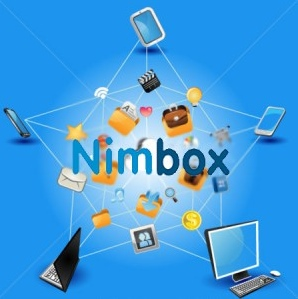
\includegraphics[width=15cm]{./Imagenes/BIimagen20}
	\end{center}


\subsection{Aplicaciones de BuBusiness Analitycs } \label{sec:nada}


\subsubsection{Aplicacion1: }\label{sec:nada2}  

\begin{center}
\caption\textbf{HERRAMIENTAS DE BUSINESS ANALITYCS}
\end{center}
\\
\\
Toda empresa necesita un plan de negocio. Muchos emprendedores caen en la tentación de poner en marcha su negocio sin analizar nada previamente y se limitan a cruzar los dedos esperando que salga bien. Y podría ser que sí, pero lo más probable es que no.\\
Lo ideal es llevar a cabo un análisis previo pormenorizado del sector y el mercado en el que pensamos adentrarnos. Hay numerosas herramientas de análisis estratégico gratuitas que nos pueden servir para para identificar qué distingue nuestra marca del resto y elaborar un buen plan de negocio para nuestra futura empresa. Estas son algunas de ellas.  
\\
\begin{itemize}
\item Análisis PEST
\\Con esta herramienta de análisis estratégico podremos analizar el entorno en el que queremos crear o establecer nuestra empresa, negocio o proyecto. Nos permite identificar posibles cambios de escenario en nuestro sector o en la región para detectar y aprovechar posibles oportunidades de crecimiento. El nombre es un acrónimo de cuatro factores:

Políticos: estabilidad política, la posibilidad de un cambio de gobierno que de lugar a cambios en las políticas fiscales o en materia de subvenciones, posibles cambios en los tratados comerciales, existencia o no de grupos de presión.
Económicos: economía en crecimiento o en recesión, tendencia del consumo, situación de confianza o de inestabilidad, los tipos de cambio, el nivel de inflacción…
Socioculturales: hábitos sociales, cambios en los gustos o en las modas de la gente, formas de comunicación habituales, demografía, salud, valores.
Tecnológicos: tecnología actual, posibles avances, desarrollos en marcha, conocimientos, inversión en I+D, información.
Debemos analizar en qué medida cada uno de estos factores macroambientales podría influir positiva o negativamente en nuestra empresa.  
		\begin{center}
		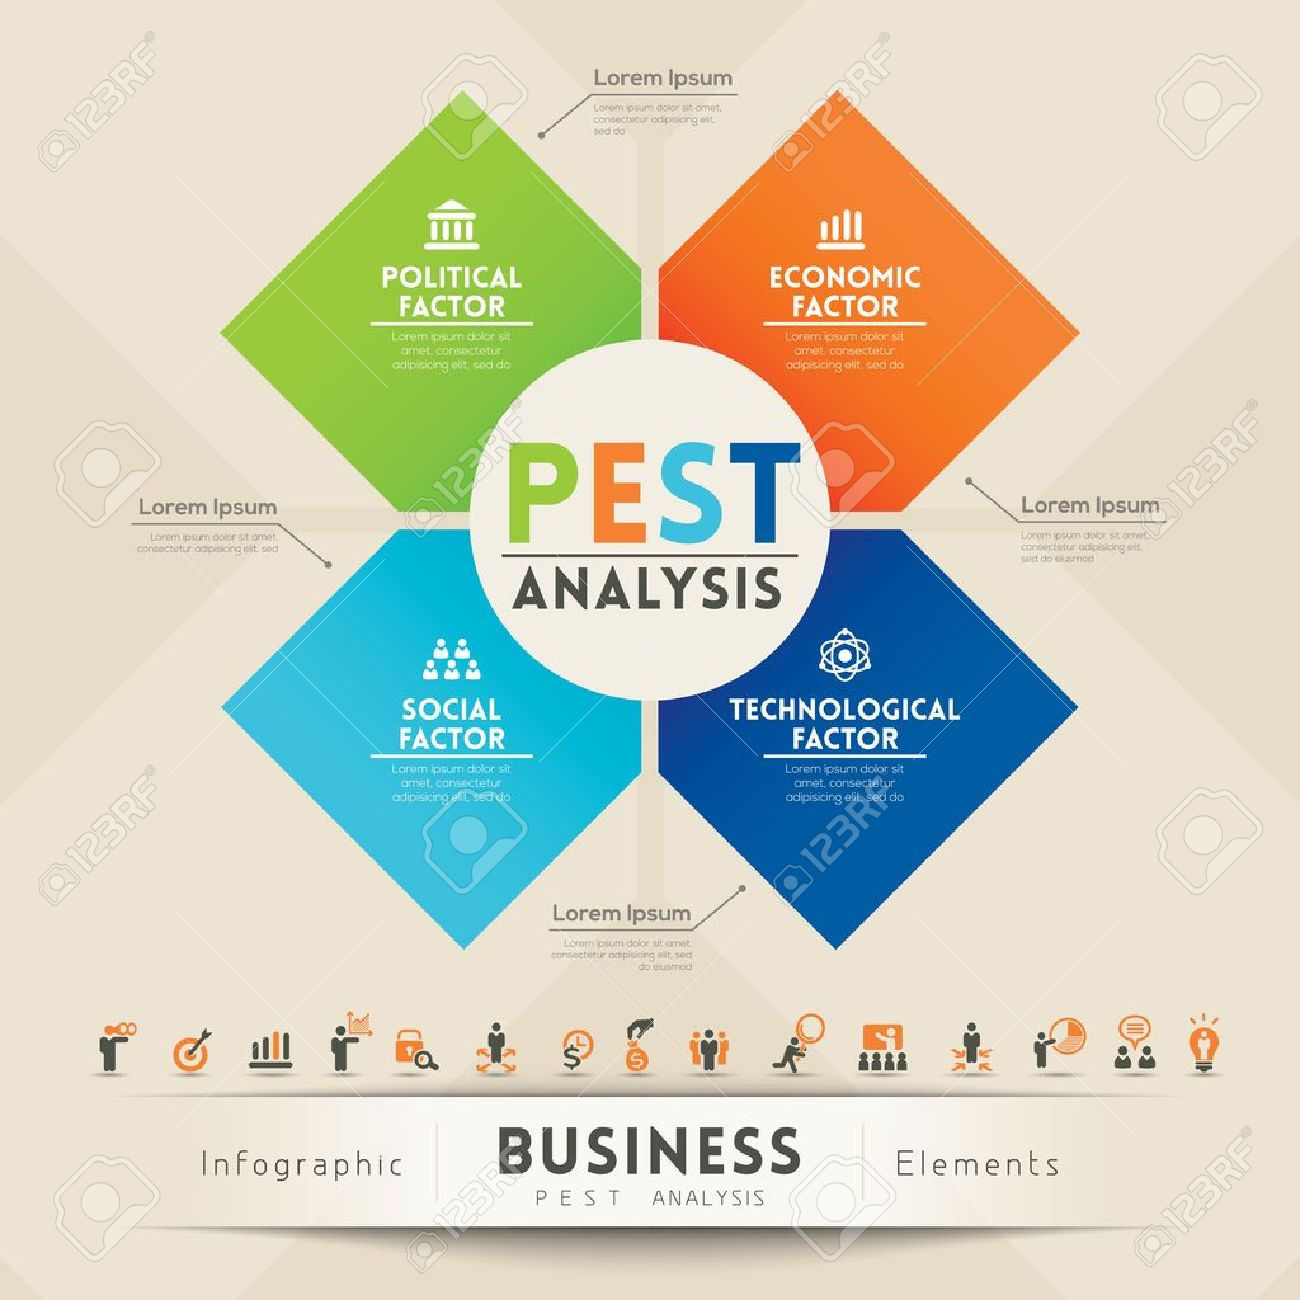
\includegraphics[width=15cm]{./Imagenes/Imagen1}
		\end{center}

	\end{itemize} 
	
	\begin{itemize}
\item Análisis PESTEL
\\Es una variación del anterior que añade dos factores más a los cuatro del análisis PEST. Además de tener en cuenta los factores políticos, económicos, sociales y tecnológicos, se analizarán también los factores:

Ecológicos: por ejemplo, el cambio climático puede tener consecuencias en diversos sectores como el turístico o el de las aseguradoras. Las leyes de protección medioambiental o las regulaciones en materia de gestión de residuos o de energías también pueden influir en una empresa.
Legales: leyes contra la discriminación, leyes de defensa del consumidor, leyes antimonopolio, licencias, legislación laboral, leyes de protección de la salud, sectores con una protección especial.
		\begin{center}
		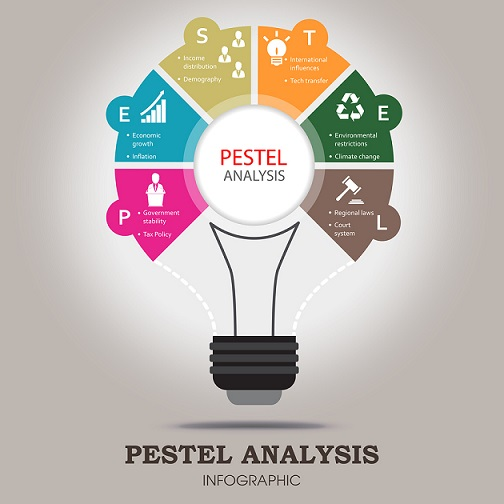
\includegraphics[width=15cm]{./Imagenes/Imagen2}
		\end{center}
	\end{itemize} 
\\
\begin{itemize}
\item Análisis FODA:
\\Es una herramienta de análisis estratégico que nos permite analizar la situación interna y externa de una empresa o proyecto. Es como hacer una fotografía de la situación de nuestra empresa. Por eso, dado que esta situación no es estático, sino que evoluciona continuamente a lo largo del tiempo, además de utilizarlo para elaborar el plan de negocio de nuestra empresa, es bueno repetirlo posteriormente cada cierto tiempo. El objetivo es conocer la situación real en la que se encuentra la organización, empresa o proyecto en cada momento y, en función de ello, planear la estrategia de futuro más adecuada. El nombre de esta herramienta de análisis es un acrónimo de Fortalezas, Oportunidades, Debilidades y Amenazas. 
		\begin{center}
		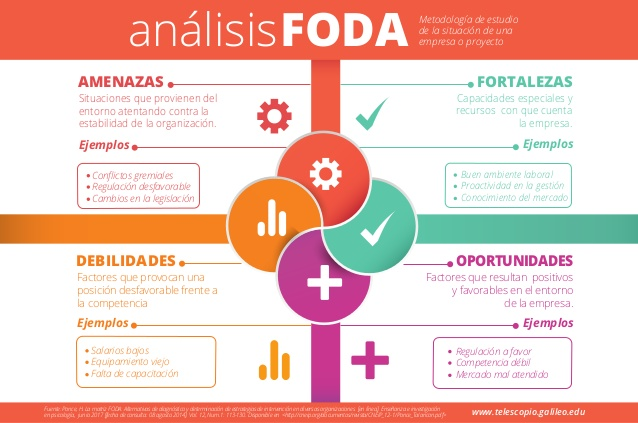
\includegraphics[width=15cm]{./Imagenes/Imagen3}
		\end{center}

	\end{itemize} 
	
	\begin{itemize}
\item Modelo de las 7 S:
\\A diferencia de la mayoría de las herramientas de análisis estratégico que suelen centrarse en el análisis externo, el Modelo de las 7 S, desarrollado a principios de los años 80 por Tom Peters y Robert Waterman, dos consultores de la firma McKinsey & Company, apunta directamente al interior de nuestra compañía. El modelo analiza, concretamente, 7 factores, cuyos nombres en inglés empiezan por S (de ahí el nombre de la herramienta, las 7 S) y que, según sus autores, son los 7 factores fundamentales de cualquier estructura organizativa:

- Estrategia (Strategy)\\
- Estructura (Structure)\\
- Sistemas (Systems)\\
- Estilo (Style)\\
- Valores compartidos (Shared values)\\
- Personal (Staff)\\
- Habilidades (Skills)
La idea del modelo es que las organizaciones no operan como un conjunto de silos estancos, sino más bien como una red de piezas interconectadas. Por eso es fundamental que los siete factores recogidos en el modelo estén alineados para que nuestra empresa tenga éxito. En este sentido, a la hora de implementar cualquier nueva estrategia, se deberá comprobar previamente todos ellos mantendrían su alineación, una vez implementada. Si la respuesta es que no para todos o parte de los factores, será necesario replantearse parte o la totalidad de la estrategia antes de proceder a su implementación. Para verlo más claro, lo mejor es dibujar un octógono y colocar cada una de las S en uno de sus vértices. Excepto los valores compartidos que, como son compartidos, los situaremos en el centro del octógono. Después, trazaremos líneas que vayan desde cada vértice hasta los demás.
		\begin{center}
		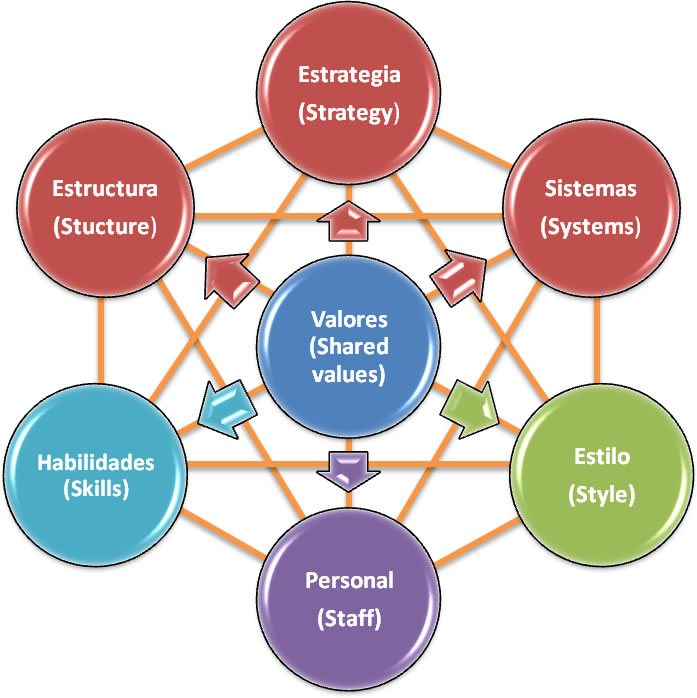
\includegraphics[width=15cm]{./Imagenes/Imagen4}
		\end{center}
	\end{itemize}
	
	\\
\begin{itemize}
\item Las 5 fuerzas de Porter:
\\Esta herramienta de análisis estratégico, ideada por el ingeniero y profesor Michael Porter en 1979, todavía sigue vigente. El modelo delimita un marco que nos permite analizar el nivel de competencia dentro de un sector para poder idear, así, una estrategia de negocio que haga rentable nuestra empresa. En este sentido, es ideal para elaborar un plan de negocio, dado que es fundamental analizar la competencia antes de crear una empresa, por lo que este modelo es especialmente interesante para emprendedores. Las cinco fuerzas de Porter son las siguientes:

- Poder de negociación de los compradores o clientes
- Poder de negociación de los proveedores o vendedores
- Amenaza de nuevos competidores
- Amenaza de productos sustitutos
- Rivalidad entre los competidores
		\begin{center}
		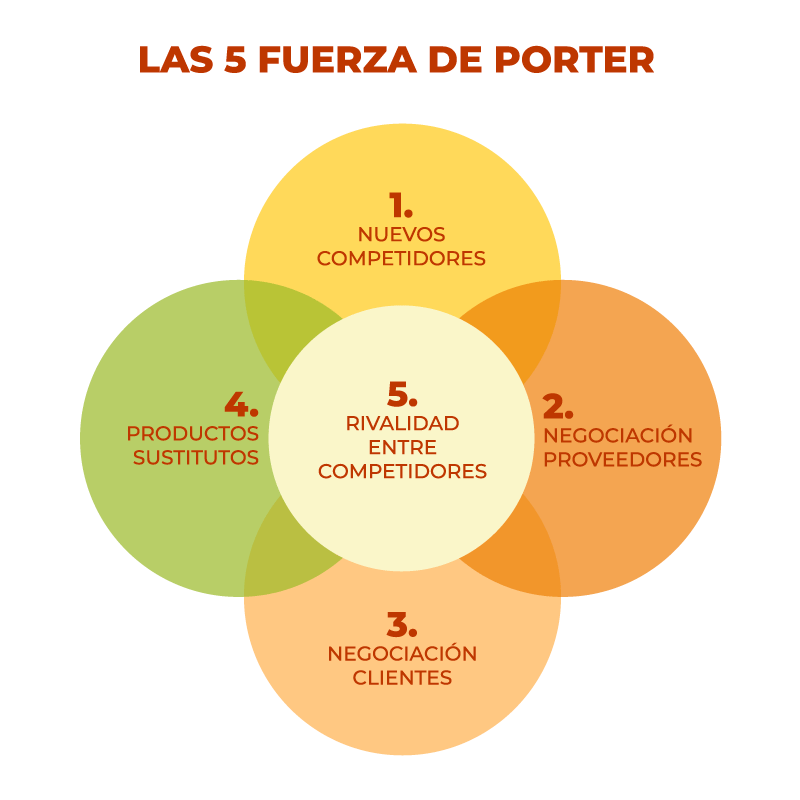
\includegraphics[width=15cm]{./Imagenes/Imagen5}
		\end{center}

	\end{itemize} 
	
	\begin{itemize}
\item Estrategia del océano azul:
\\Esta herramienta, más que para elaborar nuestro plan de negocio, es ideal para hacernos pensar y ver cómo queremos enfocar nuestra empresa. Una estrategia de océano azul es lo que puede llevar nuestra empresa al éxito. Por eso todo emprendedor debería conocer esta herramienta y, antes de montar su empresa soñada, dedicar un tiempo a pensar cuál puede ser su estrategia del océano azul.
		\begin{center}
		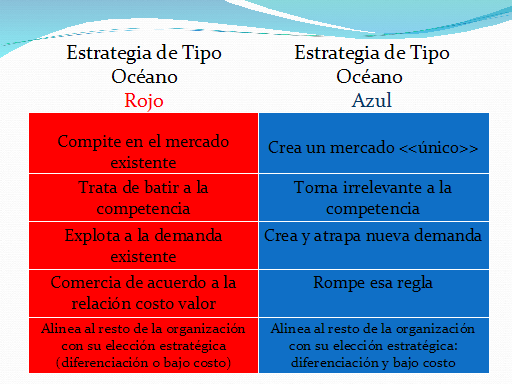
\includegraphics[width=15cm]{./Imagenes/Imagen6}
		\end{center}
	\end{itemize} 
	
\section{Conclusiones}
\\
\itemSe solía decir que la información es poder. Pero ahora el poder es entenderla. Por eso cualquier empresa hoy en día debería plantearse seriamente el uso de herramientas de análisis de datos para extraer todo el conocimiento posible de su organización. Solo así podrá mantenerse competitiva en el mercado.
\\
\item En forma exclusiva, la inteligencia empresarial y el análisis de negocios forman los componentes esenciales requeridos por una empresa para administrar su información de manera efectiva.
\\
\item 
Las dos terminologías parecen tener similitudes de una manera que hace que los estudiantes deduzcan que están conectados. De hecho, vale la pena reconocer que la analítica es una función de la inteligencia empresarial. La información analizada mediante análisis para predecir el futuro es la misma información obtenida del componente de inteligencia de la empresa. Tanto BI como BA se enfocan en impulsar a la compañía a avanzar enérgicamente
\\
\item En un medio globalizado y audaz como el del mundo empresarial, podemos ver que el entorno en el que la inmensa mayoría de las empresas tiene soportados los procesos de negocio con diferentes sistemas de información y estrategias, los ubica en un mercado tan competitivo como el actual, Hoy se ha convertido en un problema, por lo que la Inteligencia de Negocios se erige como una pieza clave para ser proactivo a la hora de tomar mejores decisiones y de conseguir mejor control de negocio y ventajas que nos diferencien de la competencia.
\\
\item Lo que HEMOS APRENDIDO es que la gran mayoría de empresas no utilizan sistemas de inteligencia empresarial para gestionar sus negocios. Sin embargo, SABEMOS QUE SI ENTIENDEN EL CONCEPTO, y saben que son herramientas muy enriquecedoras para la gestión actual, a lo que añaden las siguientes ventajas para el  uso de Software de Inteligencia de Negocios:

 – Los sistemas de Business Intelligence ayudan a hacer más competitiva la estrategia de la empresa.

 – Apoyan la toma de decisiones que son vitales para obtener mejores resultados

 – La Inteligencia de Negocios facilita notablemente la interactividad entre usuarios, clientes y proveedores.

 – Facilitan el acceso a los datos críticos de la empresa y las informaciones corporativas para la integración de datos y la toma de decisiones

 – Permite alinear acciones de diferentes departamentos e igualmente ayuda a controlar cada línea de negocio o departamento con métricas específicas.
 \\

(\ref{eq:area}).
También se pueden mencionar secciones de la misma forma: ver sección
\ref{sec:nada}. O citar algo de la bibliografía: \cite{Cd94}.


% Bibliografía.
%-----------------------------------------------------------------
\begin{thebibliography}{99}

\bibitem{Cd94} https://selecthub.com/business-intelligence/business-intelligence-vs-business-analytics/
\\
\bibitem{Cd94} https://www.betterbuys.com/bi/business-intelligence-vs-business-analytics/
\\
\bibitem{Cd94} https://aprendebi.wordpress.com/2016/11/30/bussiness-intelligence-vs-bussiness-analytics/
\\
\bibitem{Cd94} http://scholarium.info/analisis-de-negocio-business-analysis-ba/
\\
\bibitem{Cd94} https://blog.corponet.com.mx/que-es-la-inteligencia-de-negocios

\end{thebibliography}

\end{document}
